\section{Auswertung}

\subsection{Gegenfeldmethode}

Bei   dieser   Messung  wird  nach  der  Gegenfeldmethode  vorgegangen.   Jede
Spektrallinie der Hg-Dampf-Lampe wird isoliert und die gegenspannung sowie die
Photospannung wird bestummen.

Es ist im dunklen gut ersichtlich, wie  die  Spektrallinien der Hg-Dampf-Lampe
zerlegt  werden.  Dies   ist   in   der   Abbildung   \ref{fig:spektrallinien}
ersichtlicht.

\begin{figure}[H]
    \centering
    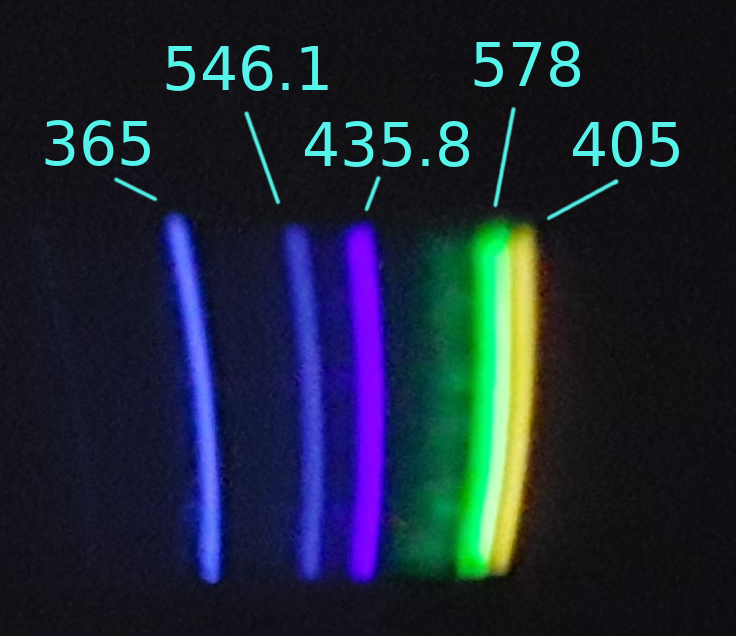
\includegraphics[width=.4\linewidth]{images/hg-spektrallinien.png}
    \caption{Spektrallinien der Hg-Dampf-Lampe und deren Wellenl\"angen}
    \label{fig:spektrallinien}
\end{figure}

Es  wurden  jeweils   die  Photospannung  und  die  Gegenspannung  der  f\"unf
spektrallinien   der   Hg-Dampf-Lampe   gemessen   und   in  den   Abbildungen
\ref{fig:photospannung}  und  \ref{fig:gegenspannung} in Funktion der Frequenz
eingetragen.

\begin{figure}[H]
    \centering
    \begin{subfigure}{.45\linewidth}
        \centering
        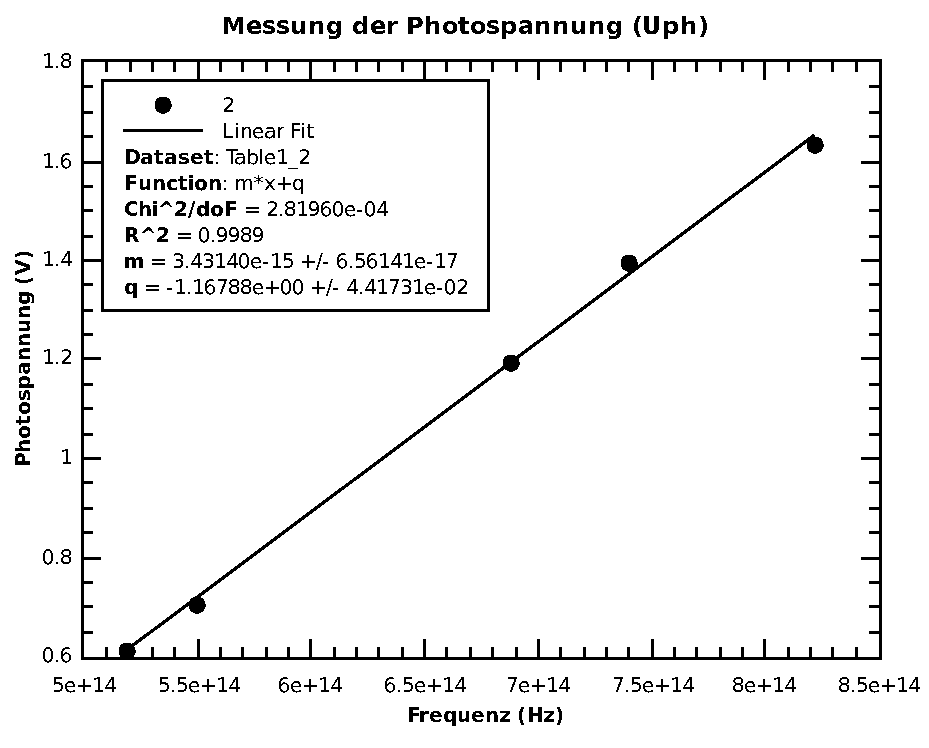
\includegraphics[width=\linewidth]{images/photospannung}
        \caption{Messung der Photospannung $U_{ph}$}
        \label{fig:photospannung}
    \end{subfigure}
    \begin{subfigure}{.45\linewidth}
        \centering
        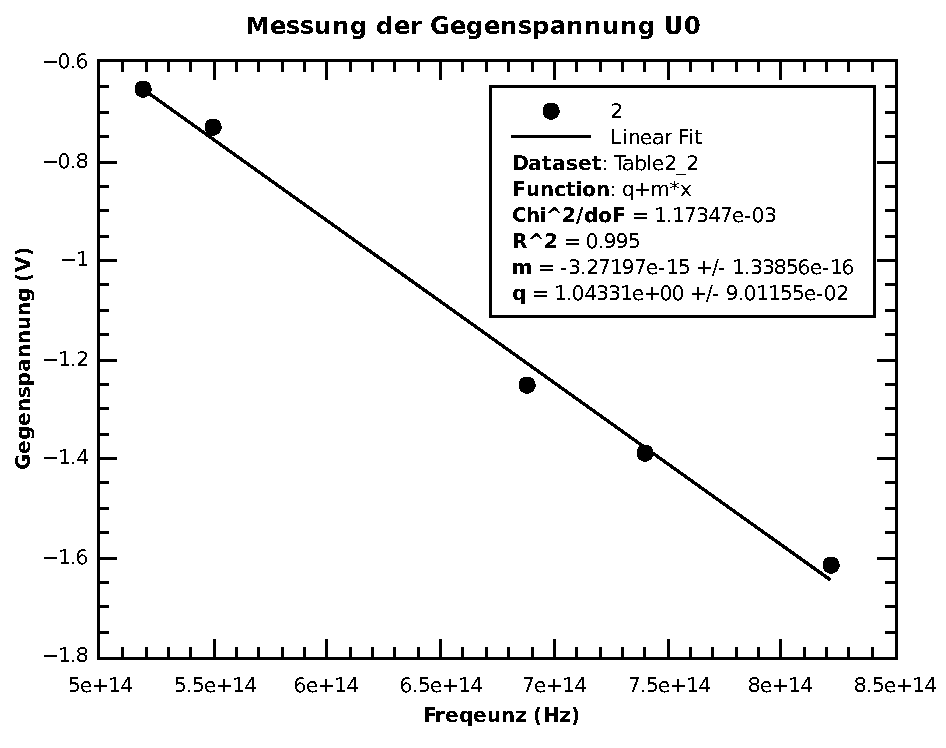
\includegraphics[width=\linewidth]{images/gegenspannung}
        \caption{Messung der Gegenspannung $U_0$}
        \label{fig:gegenspannung}
    \end{subfigure}
\end{figure}

Aus einer  linearen  Regression werden die Steigungen gewonnen. Das Vorzeichen
ist dabei egal. Die Steigungen sind:

\begin{align*}
    m_{ph} = \overline{m_{ph}} \pm s_{m_{ph}} &= 3.43140e-15 \pm 0.0656141e-15 \\
    m_0    = \overline{m_0} \pm s_{m_0}       &= 3.27197e-15 \pm 0.133856e-15
\end{align*}

\clearpage
\subsection{Bestimmen von h anhand der Knickspannung von LEDs}

Es waren 6 verschiedene LEDs vorhanden. Zuerst m\"ussen die Wellenl\"angen der
einzelnen LEDs bestummen werden. Die  Spektren  der  einzelnen LEDs wurden mit
Hilfe eines USB-Spektrometers und dem Programm  LoggerPro  aufgenommen und die
Peaks wurden notiert. Die Spektren sind in den Abbildungen \ref{fig:led-blue},
\ref{fig:led-green},          \ref{fig:led-orange},         \ref{fig:led-red},
\ref{fig:led-white} und \ref{fig:led-IR} zu sehen.

\begin{figure}[H]
    \centering
    \begin{subfigure}{.3\linewidth}
        \centering
        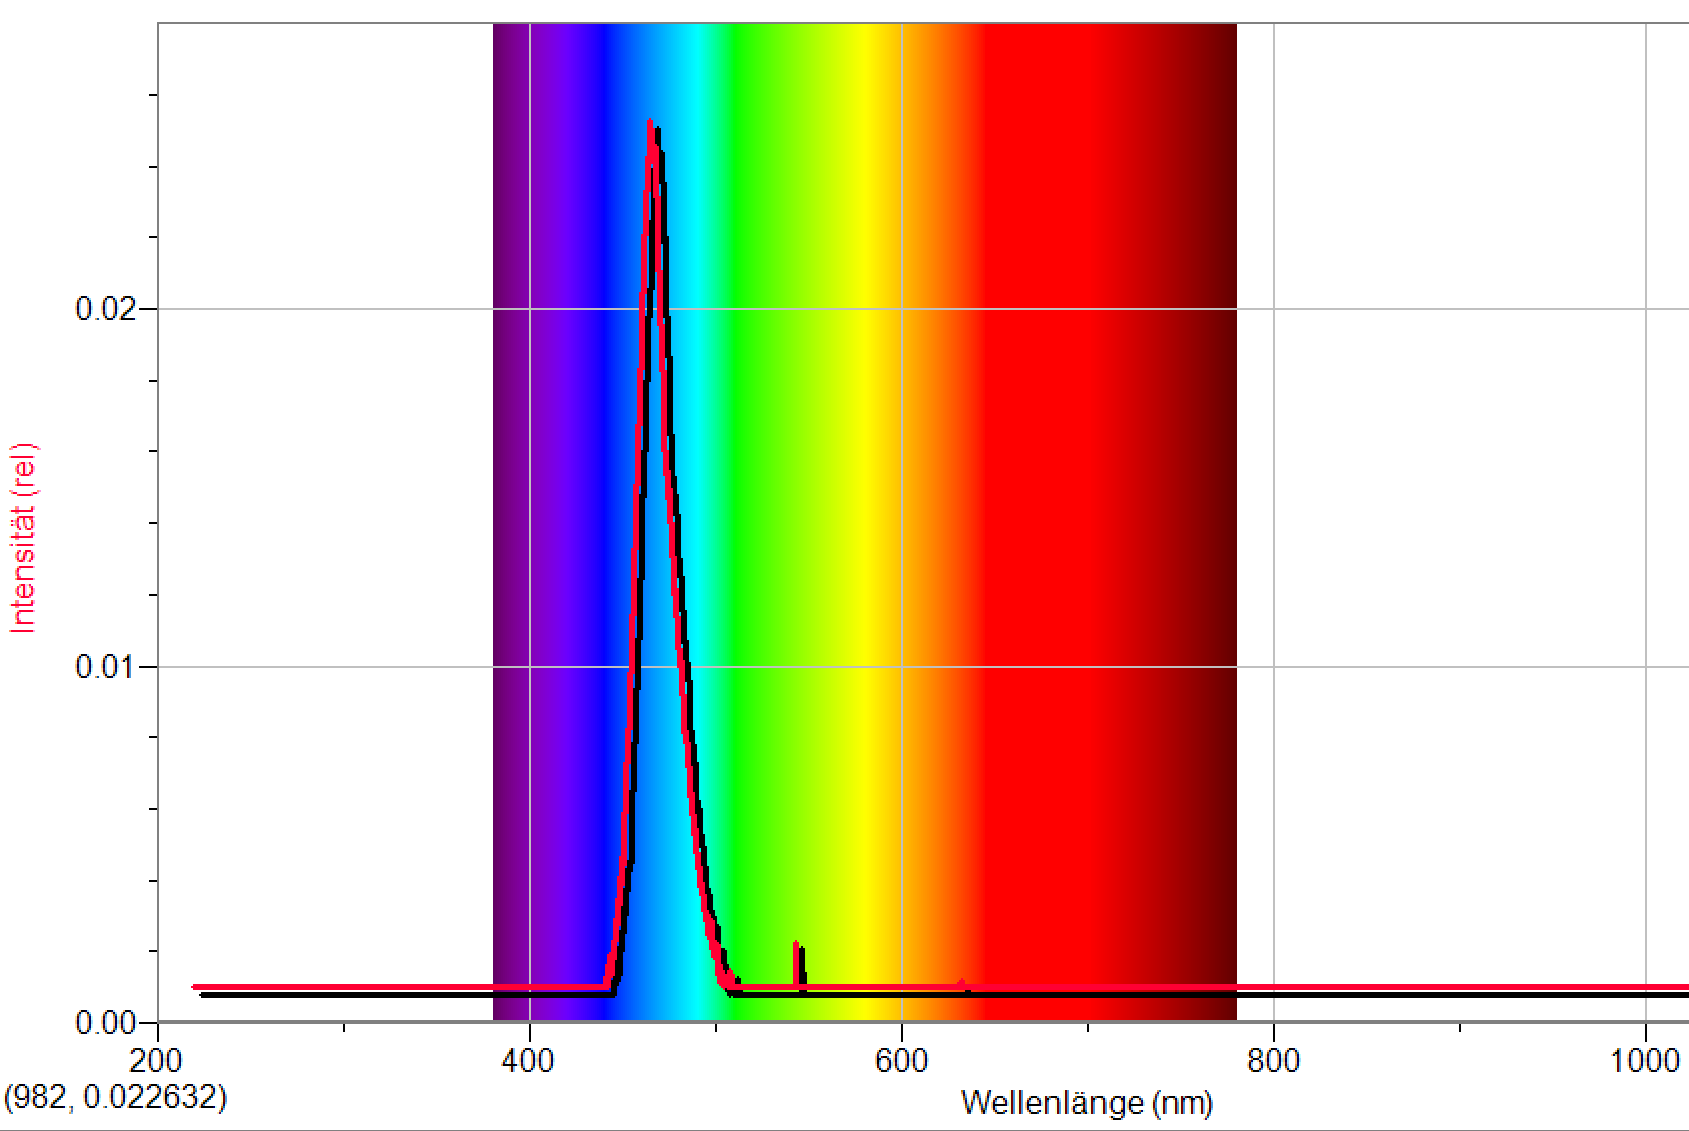
\includegraphics[width=\linewidth]{images/spectrum-blue.png}
        \caption{Spektrum des blauen LEDs, $\lambda=\SI{466.1}{\nano\meter}$}
        \label{fig:led-blue}
    \end{subfigure}
    \begin{subfigure}{.3\linewidth}
        \centering
        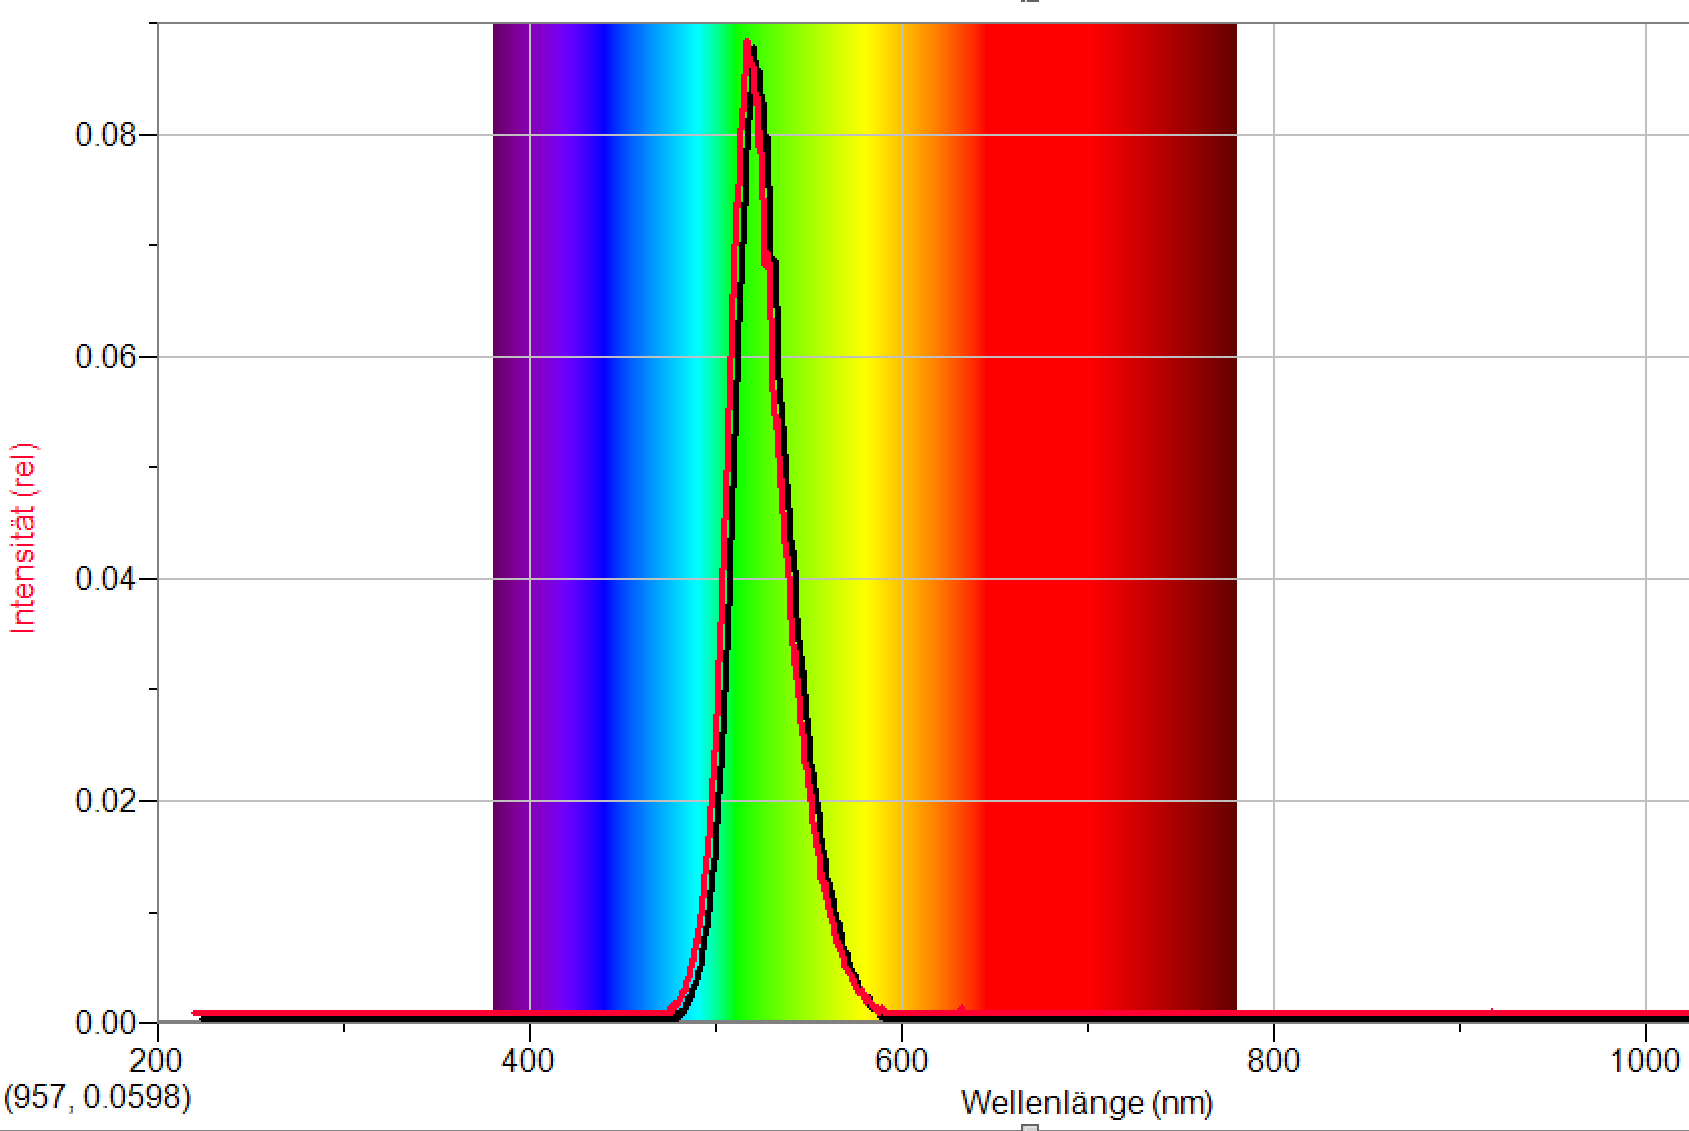
\includegraphics[width=\linewidth]{images/spectrum-green.png}
        \caption{Spektrum des gr\"unen LEDs, $\lambda=\SI{518.6}{\nano\meter}$}
        \label{fig:led-green}
    \end{subfigure}
    \begin{subfigure}{.3\linewidth}
        \centering
        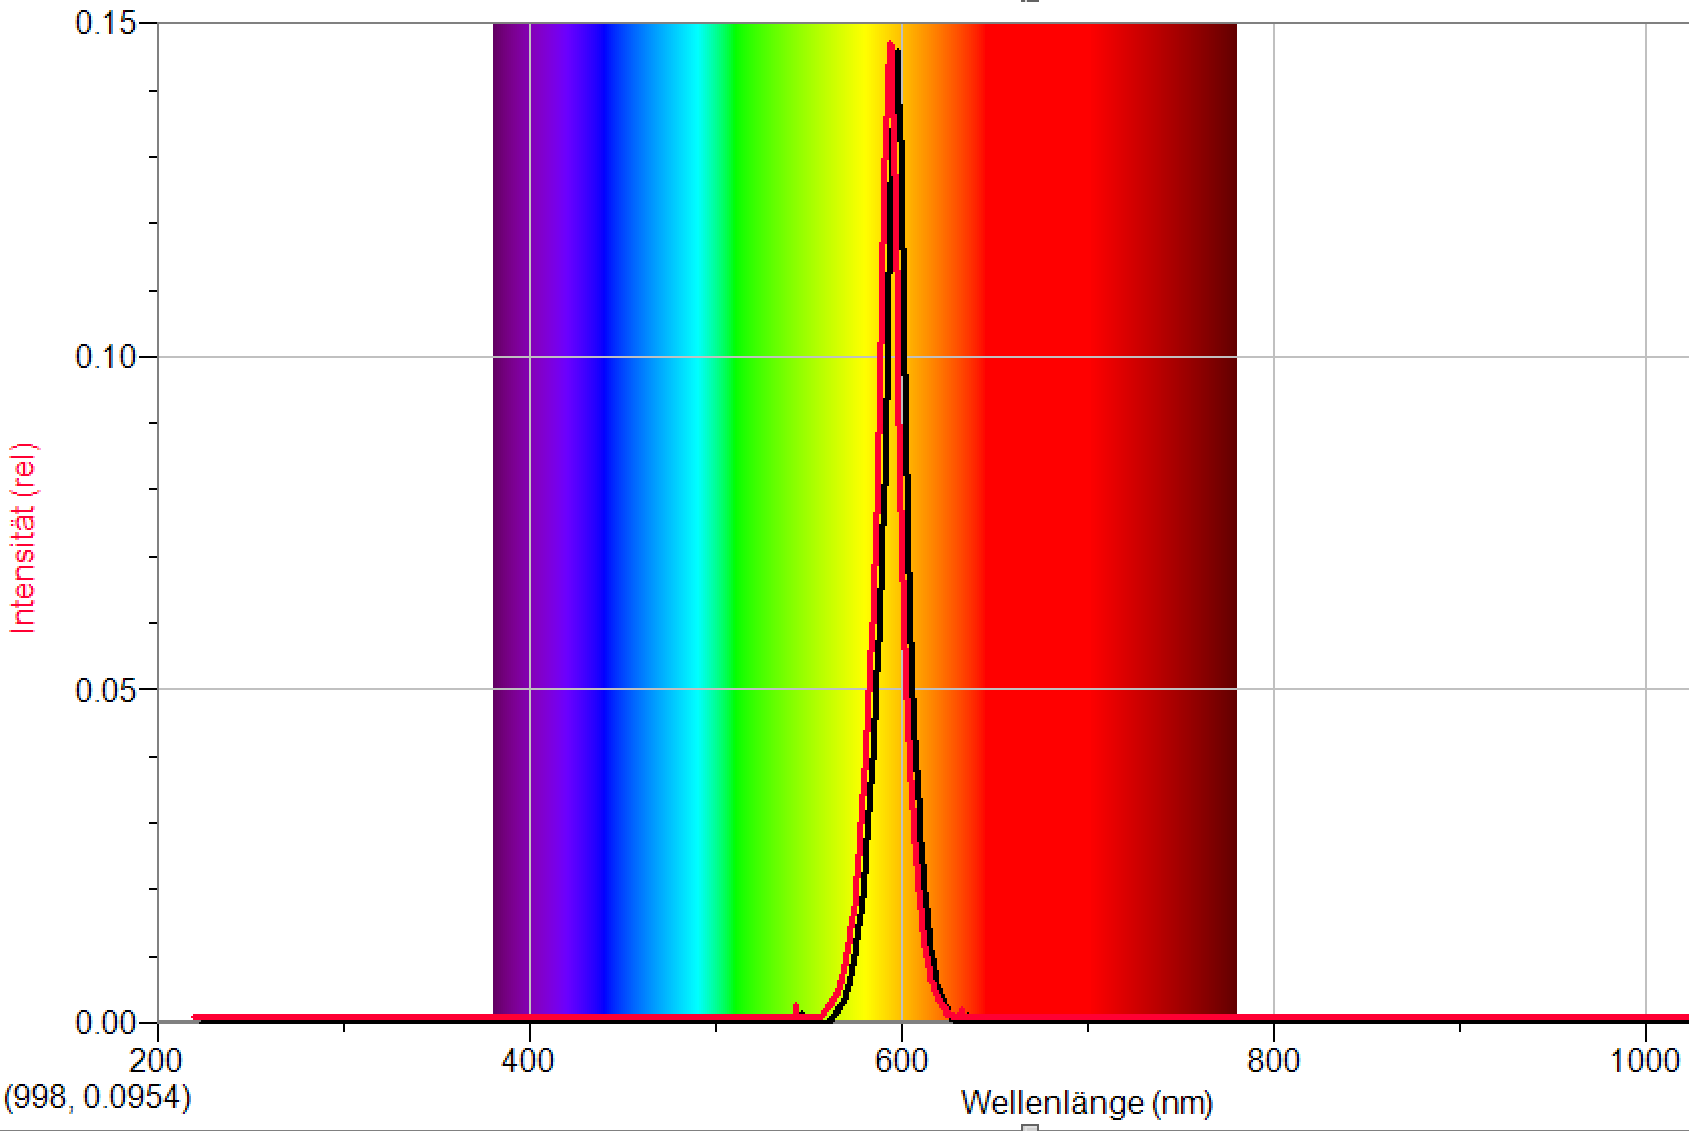
\includegraphics[width=\linewidth]{images/spectrum-orange.png}
        \caption{Spektrum des orangen LEDs, $\lambda=\SI{594.9}{\nano\meter}$}
        \label{fig:led-orange}
    \end{subfigure}
    \begin{subfigure}{.3\linewidth}
        \centering
        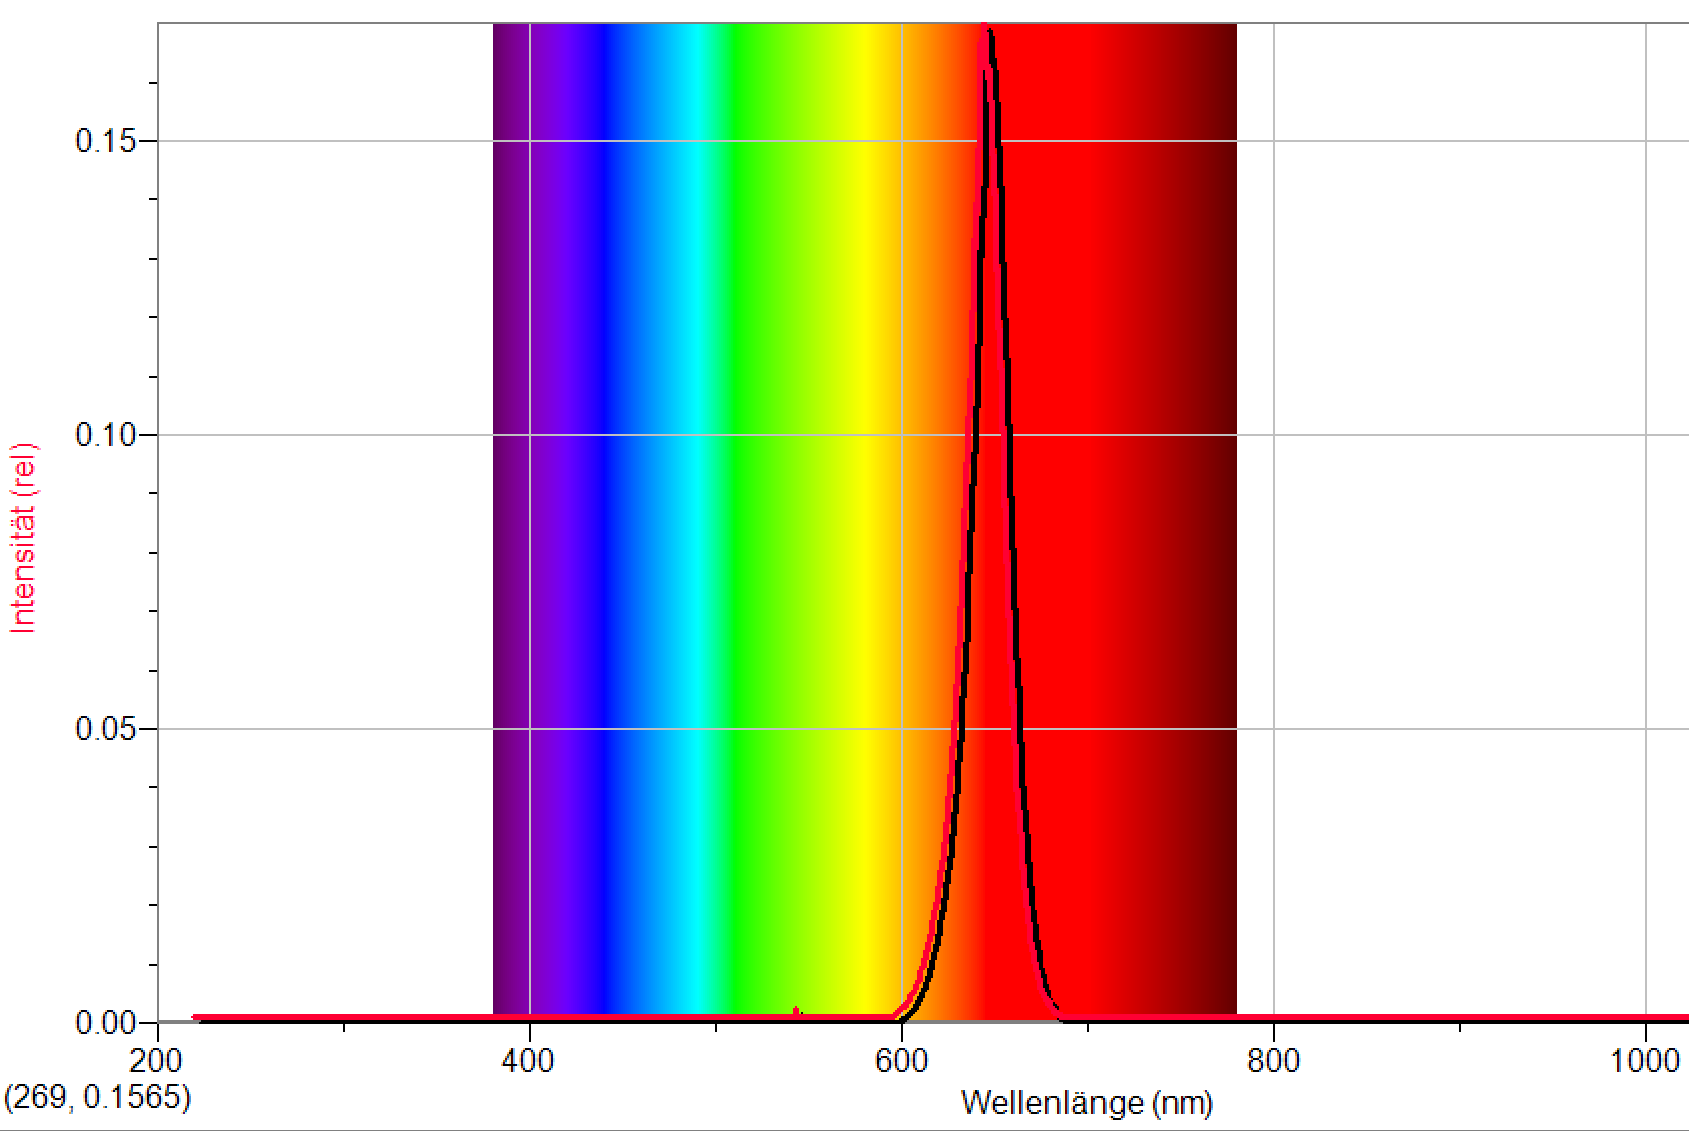
\includegraphics[width=\linewidth]{images/spectrum-red.png}
        \caption{Spektrum des roten LEDs, $\lambda=\SI{644.5}{\nano\meter}$}
        \label{fig:led-red}
    \end{subfigure}
    \begin{subfigure}{.3\linewidth}
        \centering
        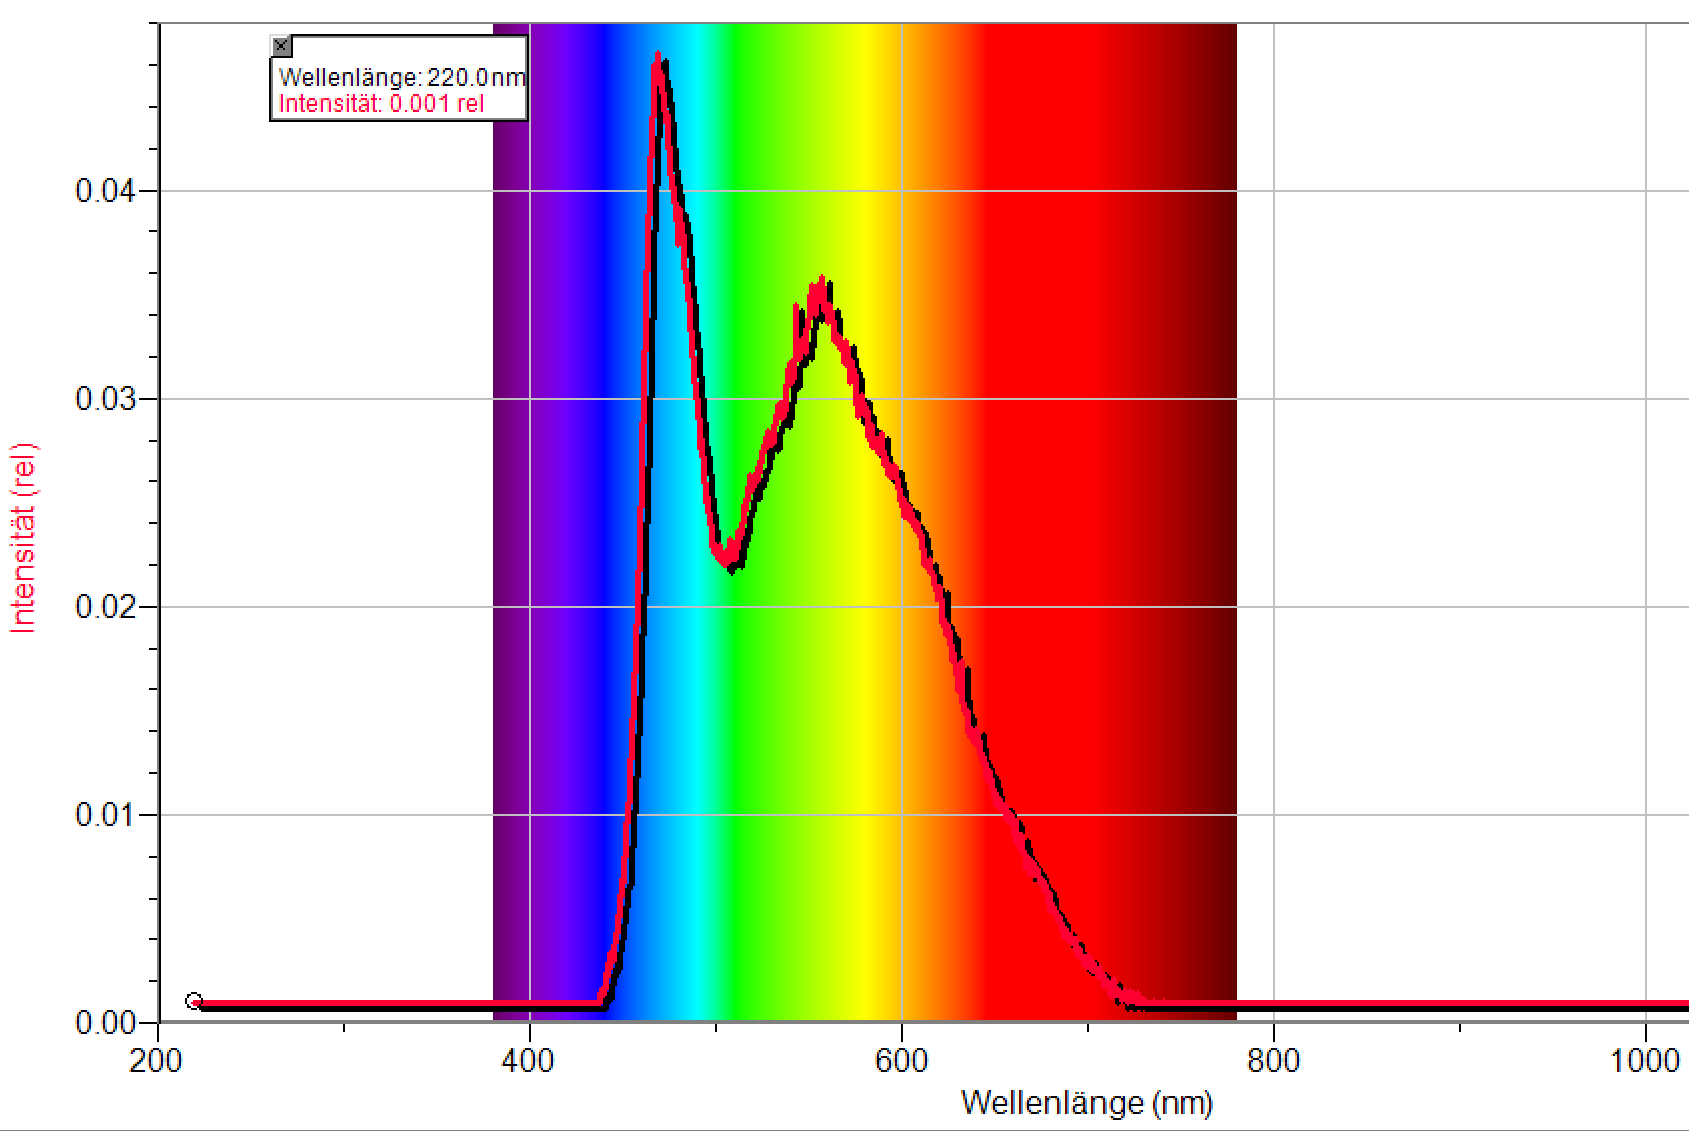
\includegraphics[width=\linewidth]{images/spectrum-white.png}
        \caption{Spektrum des weissen LEDs (hat mehrere Wellenl\"angen)}
        \label{fig:led-white}
    \end{subfigure}
    \begin{subfigure}{.3\linewidth}
        \centering
        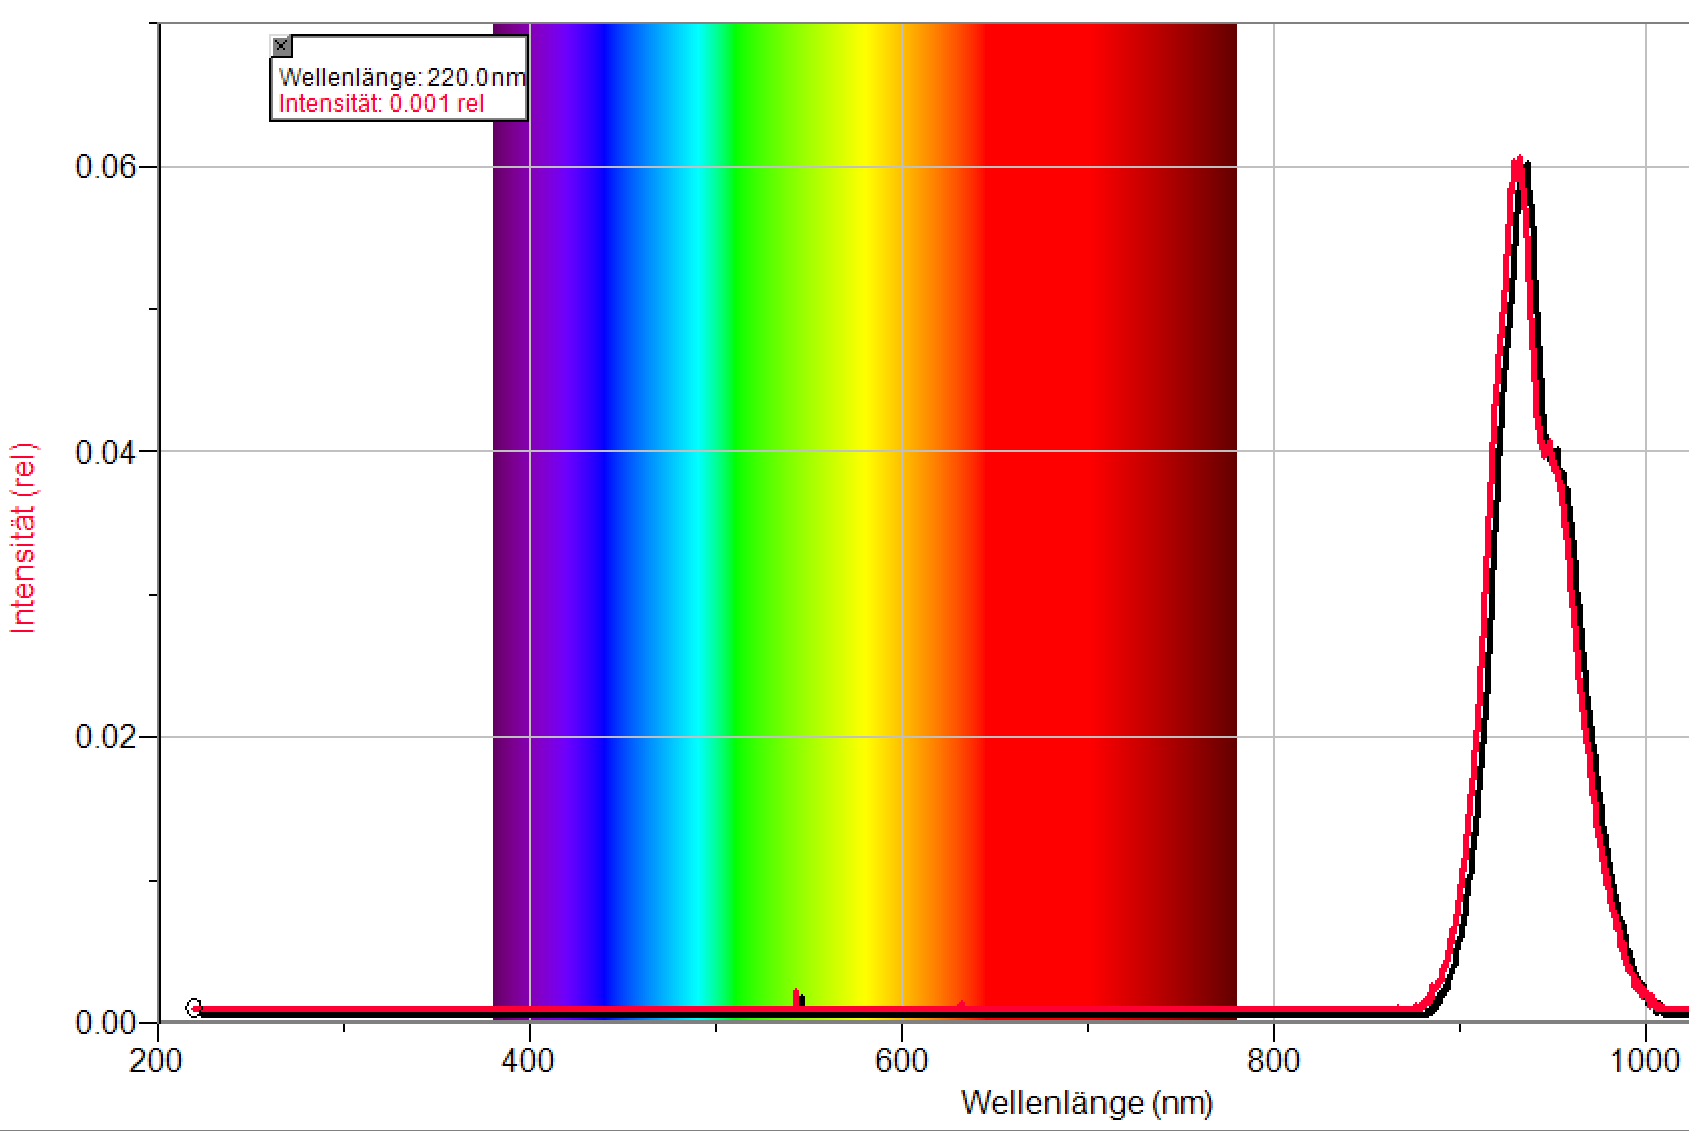
\includegraphics[width=\linewidth]{images/spectrum-IR.png}
        \caption{Spektrum des infraroten LEDs, $\lambda=\SI{931.5}{\nano\meter}$}
        \label{fig:led-IR}
    \end{subfigure}
\end{figure}

Die  weisse  LED  enth\"alt  mehrere spektrale Komponenten und hat daher keine
definierte Wellenl\"ange.

Danach wurden  die  verschiedenen LEDs an einer oszillierenden Spannung gelegt
und    eine    Spannungs-Strom-Kennlinie    aufgenommen    (siehe    Abbildung
\ref{fig:knickspannung-plot}. Die Knickspannung $U_k$  kann  daraus  bestummen
werden (siehe Abbildung \ref{fig:knickspannung}).

\begin{figure}[H]
    \centering
    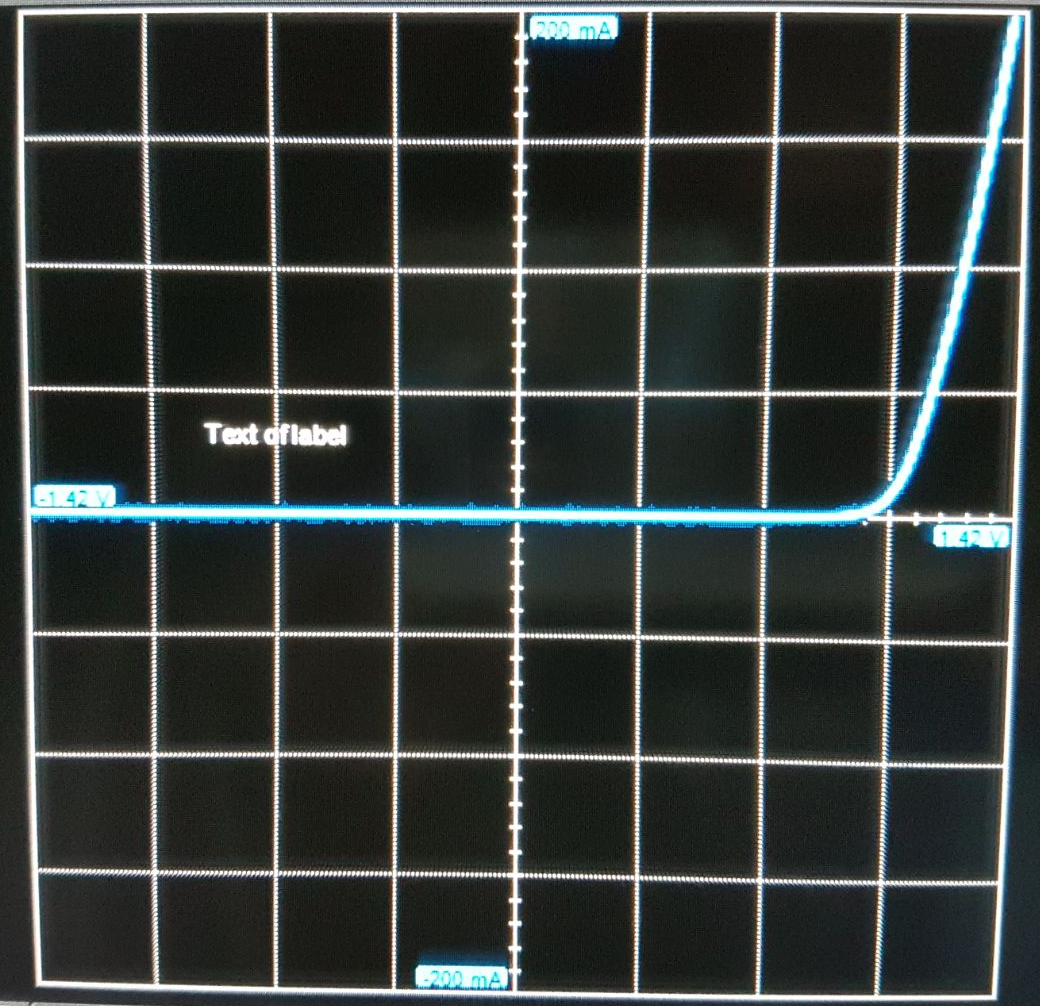
\includegraphics[width=.5\linewidth]{images/knickspannung.png}
    \caption{Messung der Knickspannung eines LEDs}
    \label{fig:knickspannung-plot}
\end{figure}

\begin{figure}[H]
    \centering
    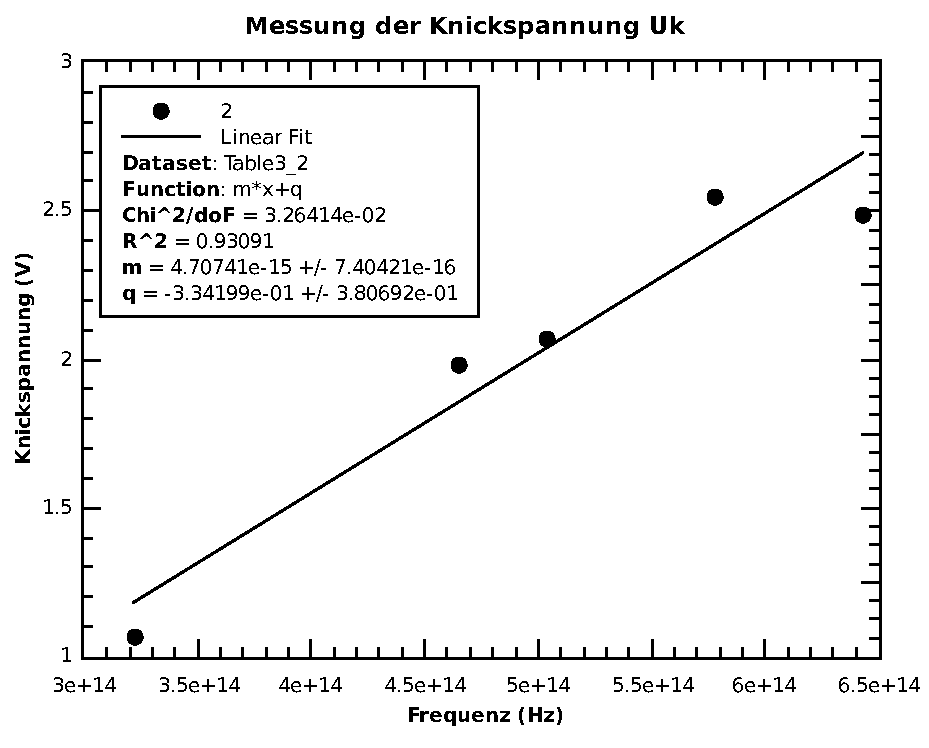
\includegraphics[width=.5\linewidth]{images/knickspannung.pdf}
    \caption{Messung der Knickspannung verschiedener LEDs}
    \label{fig:knickspannung}
\end{figure}

Die einzelnen Knickspannungen sind  in  Funktion  der  Frequenz  in  Abbildung
\ref{fig:knickspannung} dargestellt. Wieder durch lineare Regression  wird die
Steigung $m$ bestummen. Diese ist:

\begin{equation}
    m_{k} = 3239870 \pm 301223
\end{equation}

